% Apéndice Magnetismo en Aceros

\chapter{Magnetismo en Aceros.} % Main appendix title

\label{AppendixMagnetismoEnAceros} % For referencing this appendix elsewhere, use \ref{AppendixA}


%\section{Magnetismo en aceros.}


Los aceros son aleaciones de hierro y carbono a las que se suman otros elementos como: manganeso, níquel, cromo, molibdeno, boro, titanio, vanadio, tungsteno, cobalto, niobio, plomo y nitrógeno. La diferencia principal entre otras aleaciones del hierro y el acero se halla en el porcentaje del carbono; el acero es hierro con un porcentaje de carbono de entre el 0,03 \% y el 1,075 \%. El acero conserva las características metálicas del hierro en estado puro pero la adición de carbono y de otros elementos tanto metálicos como no metálicos mejora sus propiedades físico-químicas. Sin embargo si la aleación posee una concentración de carbono mayor del 1,8 \% se producen lo que se llama \emph{fundiciones} que son mucho más frágiles que el acero y no es posible forjarlas sino que deben que ser moldeadas.



%\subsection{Aceros y fundiciones al carbono.}
\section{Aceros y fundiciones al carbono.}

En el hierro puro la estructura cristalina tiene poca resistencia al avance de dislocaciones esto permite que los átomos de hierro se deslicen entre sí con relativamente poca energía, el resultado es que el hierro puro es un metal bastante dúctil. Esta ductilidad se evita agregando pequeñas cantidades de carbono (entre el 0,002\% y el 2,2 \% en peso), que actúan como agentes endurecedores, trabando la estructura cristalina al deformarla actuando como intersticiales que evitan el movimiento de las dislocaciones. Este acero base es el conocido como \emph{Acero al carbono}. sus características las podemos ver en la figura \ref{fig:DiagramaFeC}.

\begin{itemize}
	\item Hasta los 911 \textdegree C (zona límite de temperatura crítica A3), el hierro ordinario cristaliza en el sistema cúbico centrado en el cuerpo (ccb) y recibe la denominación de hierro $\alpha$ o ferrita. Es un material dúctil y maleable, ferromagnético hasta los 770 \textdegree C (temperatura de Curie a la que pierde dicha cualidad; se suele llamar también A2). La ferrita puede disolver pequeñas cantidades de carbono.
	
	\item Entre 911 y 1400 \textdegree C cristaliza en el sistema cúbico centradas en las caras (ccf) y recibe la denominación de hierro $\gamma$ o austenita. Dada su mayor compacidad la austenita se deforma con mayor facilidad y es paramagnética.
	
	\item Entre 1400 y 1538 \textdegree C cristaliza de nuevo en el sistema cúbico centrado en el cuerpo (ccb) paramagnético y recibe la denominación de hierro $\delta$, que es en esencia el mismo hierro $\alpha$ pero con un parámetro de red mayor por efecto de la temperatura.

	\item A mayor temperatura de 1538 \textdegree C, el hierro se encuentra en estado líquido.
\end{itemize}

Estos tres estados se pueden agregar en forma de Perlita y Cementita con puntos singulares de aleaciones eutécticas y eutectoides en la temperatura marcada A1.

\begin{figure}[h]
	\centering
	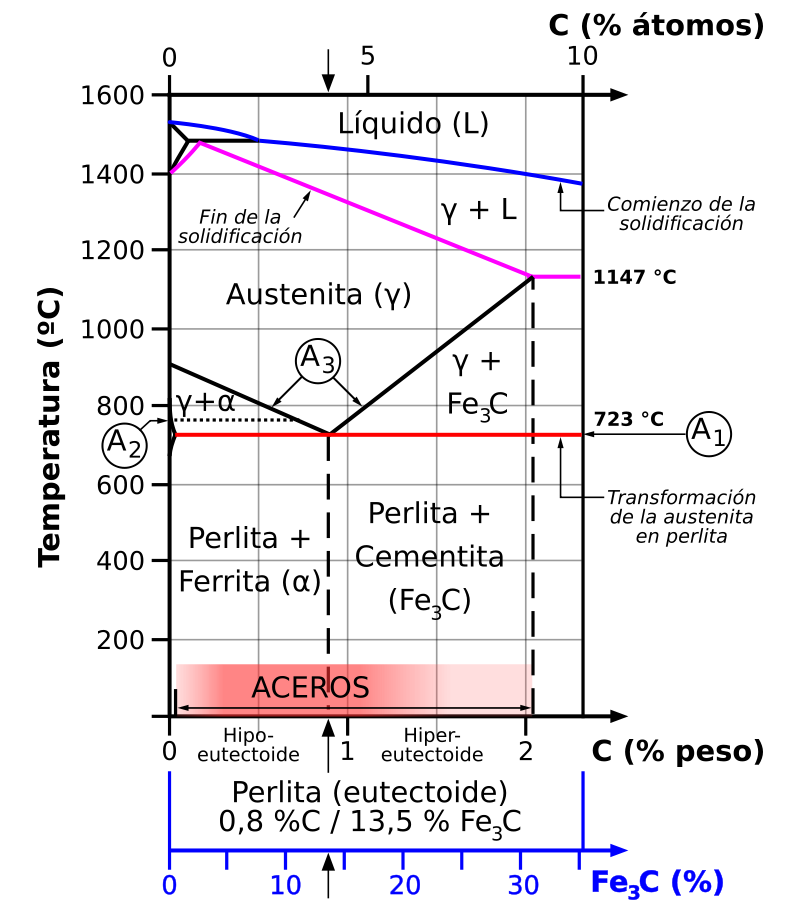
\includegraphics[width=0.75\textwidth]{./Figures/800px-Diagrama_Fe_C_zona_de_los_aceros.png}
	\caption{Diagrama de estados de acero al carbono Fe-C\protect\footnotemark.}
	\label{fig:DiagramaFeC}
\end{figure}.
\footnotetext{\url{https://es.wikipedia.org/wiki/Diagrama\_hierro-carbono}}

Si se agrega carbono al hierro aumenta su grado de ductilidad y energéticamente se ve favorecida la formación del carburo de hierro ($Fe_{3}C$) llamado cementita, que va migrando a los bordes de grano por su gran tamaño; de modo que los aceros al carbono terminan siendo conformados por ferrita y cementita como se observa en la escala inferior de la figura \ref{fig:DiagramaFeC}.

Hay estructuras que se formarán según sea el proceso de enfriamiento y el estado inicial del acero al carbono:  
\begin{itemize}
	\item La martensita es el constituyente típico de los aceros templados y se obtiene de forma casi instantánea al enfriar rápidamente la austenita (transformación de fase sin difusión). Es una solución sobresaturada de carbono en hierro $\alpha$ con la tendencia de que a mayor cantidad de carbono, más se sustituye la estructura cúbica centrada en el cuerpo (ccb) por una tetragonal centrada en el cuerpo (bct). Luego de la cementita (y los carburos de otros metales), la martensita es el constituyente más duro de los aceros.

	\item La bainita se forma a velocidades intermedias de enfriamiento, es una estructura similar a la perlita formada por agujas de ferrita y cementita pero de mayor ductilidad y resistencia que aquella.

	\item La austenita se puede retener por enfriamiento rápido de aleaciones con elementos gammágenos (que favorecen la estabilidad del hierro $\gamma$) como el níquel y el manganeso, tal es el caso de los aceros inoxidables austeníticos.
\end{itemize}

En la figura \ref{fig:FerromagnetismoParticularidad1} tenemos la capacidad calorífica a volumen constante del hierro en función de la temperatura absoluta. Podemos apreciar transiciones de fase de primer orden entre los distintos estados cristalinos del hierro $\alpha-\gamma-\delta$ y una transición de fase de segundo orden cuando dentro del mismo estado cristalino hierro-$\alpha$ el material experimenta una transición de ferromagnético a paramagnético.

\begin{figure}[h]
	\centering
	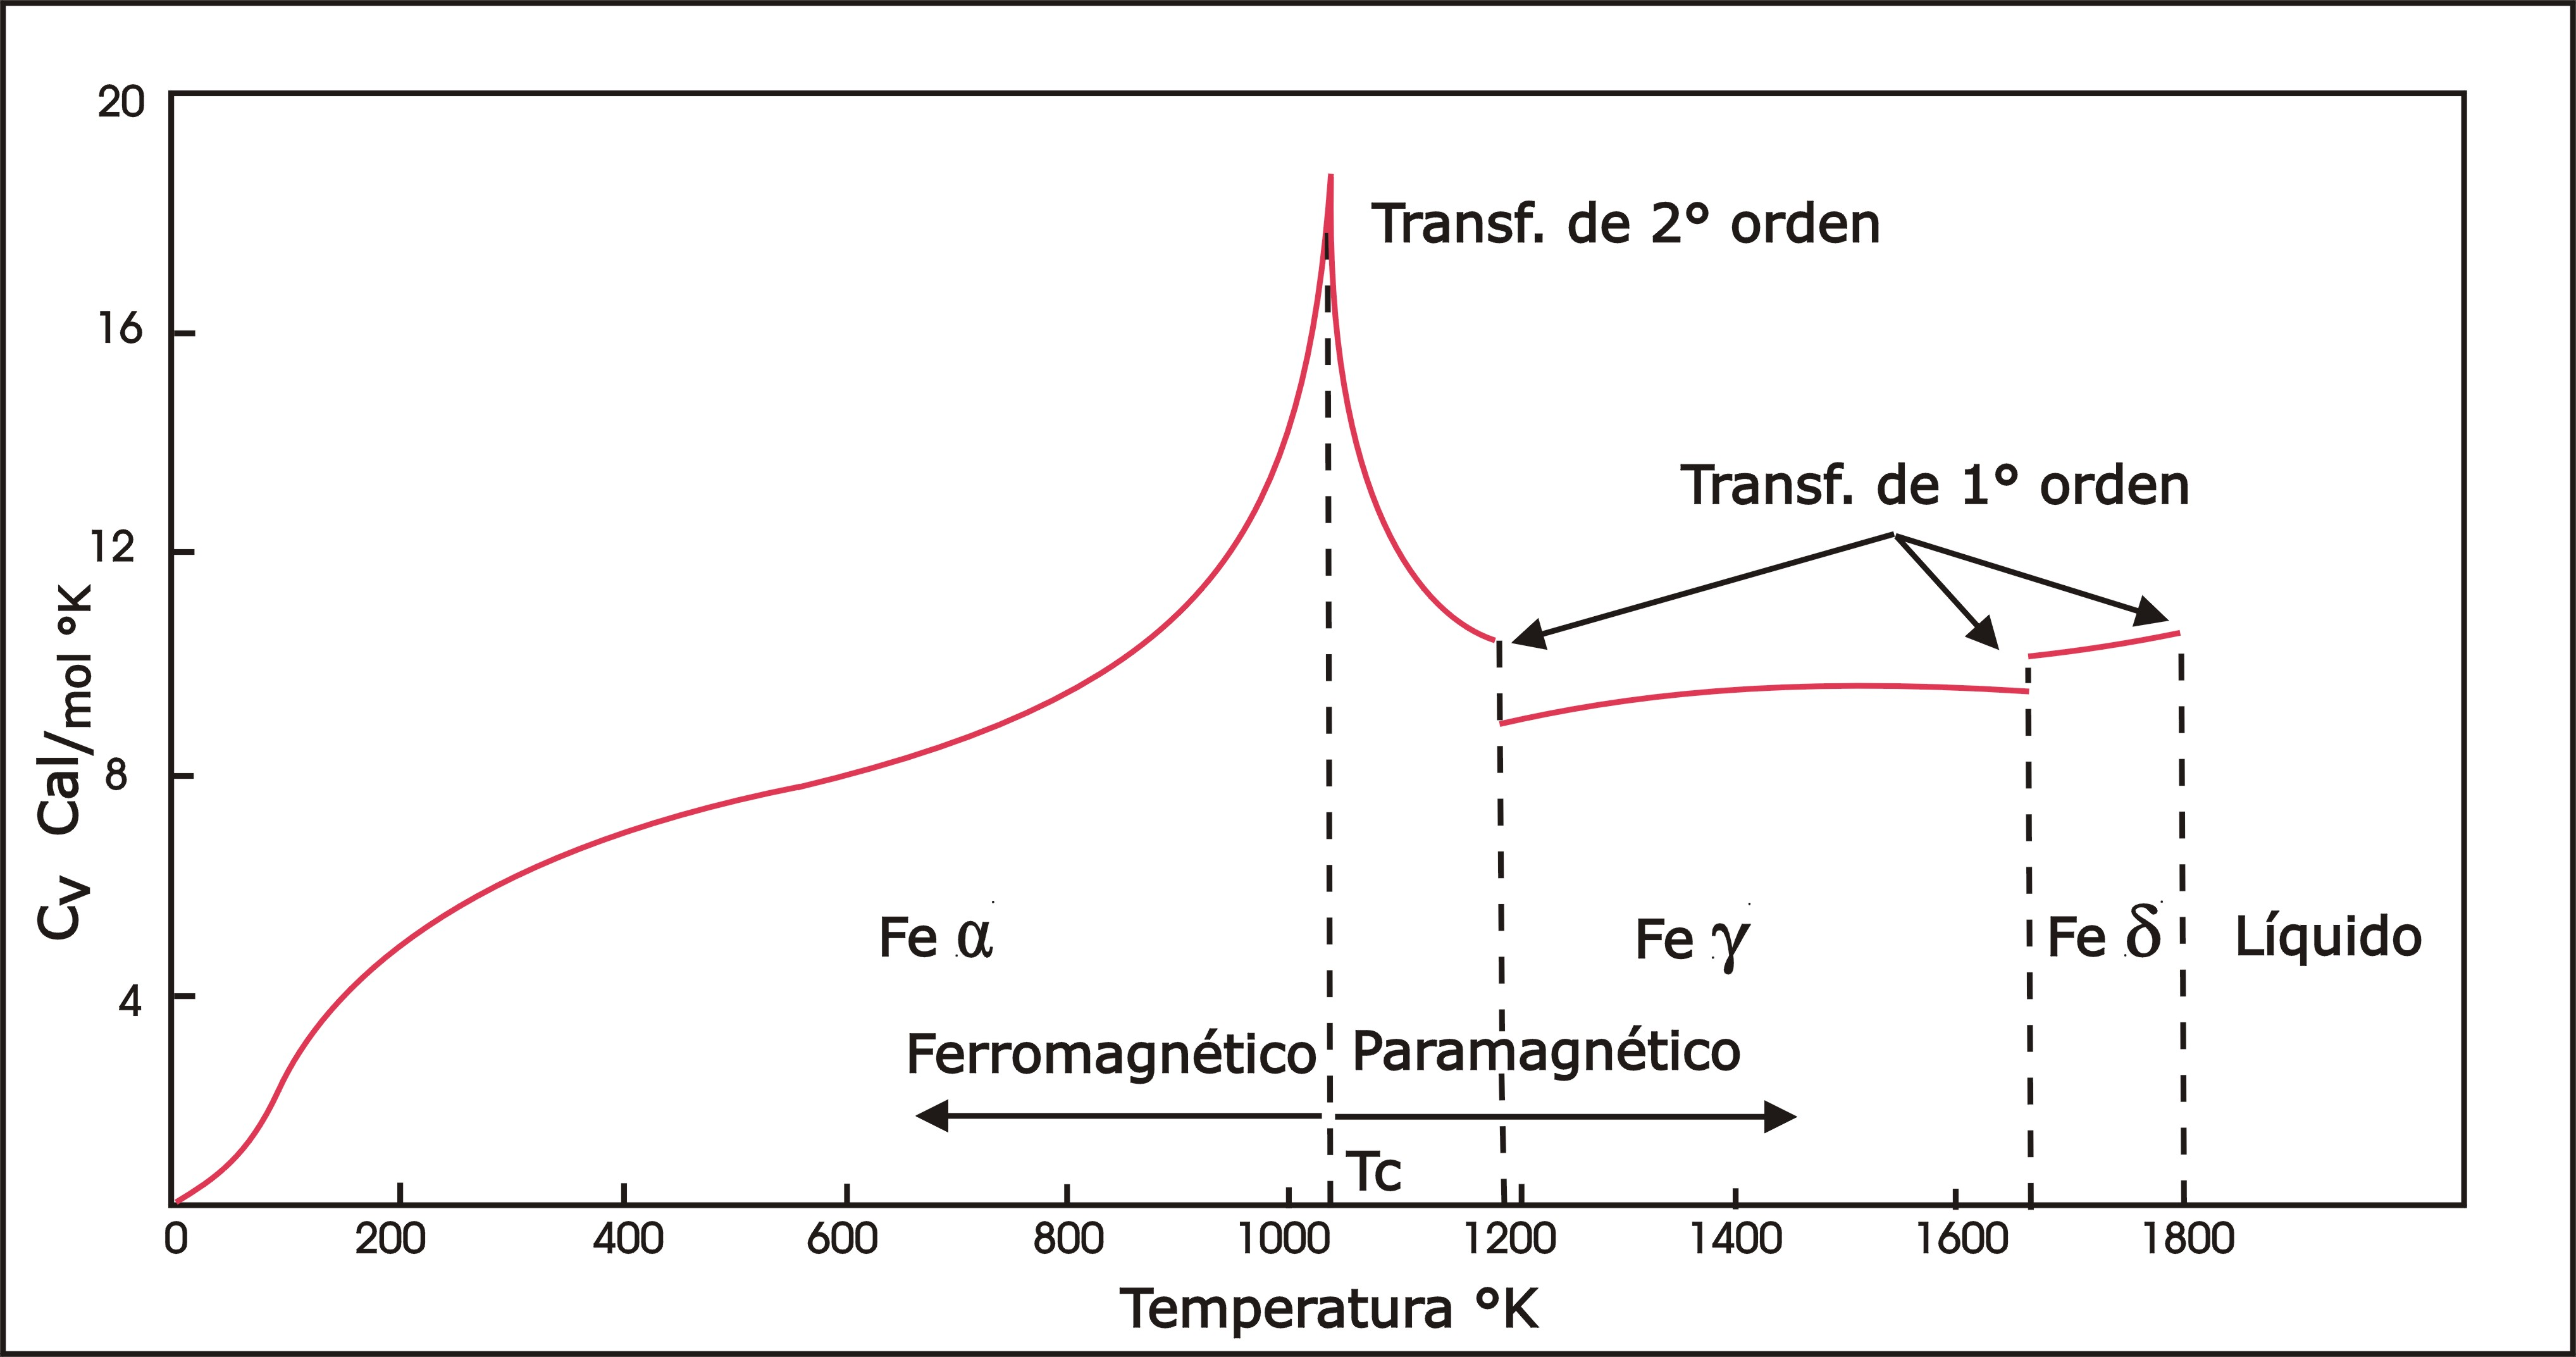
\includegraphics[width=0.90\textwidth]{./Figures/FerromagnetismoParticularidad1.jpg}
	\caption{Transiciones de fase en el Fe y cambios de estado magnético.}
	\label{fig:FerromagnetismoParticularidad1}
\end{figure}.



%\subsection{Aceros inoxidables.}
\section{Aceros inoxidables.}

El acero inoxidable es una aleación de acero compuesta de al menos un 10,5\% de cromo. Por sus características componen un grupo aparte del de los \emph{Aceros aleados} y pueden clasificar en función de los elementos que los componen cómo:

\begin{itemize}
	\item Aceros martensíticos: sólo contienen carbono y cromo. Son ferromagnéticos y fueron los primeros que se desarrollaron industrialmente. El contenido de cromo va del 10,5 al 18 \% y el de carbono hasta el 1,2\%. Se utilizan en Cuchillería, discos de freno, partes para bombas y turbinas a gas o vapor, tuercas y tornillos, equipos quirúrgicos, instrumentos dentales,  etc.
	\item Aceros ferríticos: contienen no menos 16\% de cromo y puede llegar hasta el 30\% y 0,12\% de carbono. Son ferromagnéticos y según el porcentaje de cromo y el agregado de titanio, niobio y molibdeno se dividen en cinco subgrupos. Son ampliamente usados en la industria de los equipos comerciales de alimentos, refrigeradores, bateas, reactores, tuberias, etcetera. Resistencia a la corrosión de moderada a buena, se endurecen por deformación en frio, no pueden ser endurecidos por tratamiento térmico. Son ferromagnéticos.
	\item Aceros dúplex: se denominan así por tener en su estructura metalúrgica proporciones similares de ferrita y austenita. Son ferromagnéticos y su límite elástico es casi el doble de un acero austenítico y con una resistencia a la corrosión muy similar, poseen una excelente tenacidad, superior a la de los aceros ferríticos. Se utilizan en la industria marina, especialmente en los cascos de submarinos.
	\item Aceros PH: tambien conocidos como endurecidos por precipitación y ofrecen una alternativa a los aceros inoxidables austeníticos cuando se desean elevadas características mecánicas y de maquinabilidad. Son aleaciones hierro-cromo-níquel mayormente ferromagnéticas sometidas a endurecimiento por tratamiento térmico de envejecimiento. Se pueden clasificar en función de su estructura en estado de recocido y del comportamiento resultante tras el tratamiento de envejecimiento como austeníticos, semi-austeníticos o martensíticos. Los aceros PH están patentados y frecuentemente se les designa con las siglas de la empresa fabricante. 
	\item Aceros austeníticos: caracterizados por su alta resistencia a la corrosión pueden ser ferromagnéticos o ligeramente paramagnéticos. Los clasificados según la norma AISI\footnote{\url{https://www.steel.org/}} como AISI 304 (A2) y AISI 316 (A4) presentan una estructura austenítica que se caracteriza por ser casi amagnética. Sin embargo cuando estos aceros son sometidos a procesos de deformación en frío (estampado, cizallado o laminado), la austenita sufre una transformación parcial en martensita de deformación caracterizada por una mayor dureza y por ser ferromagnética, fácilmente detectable por un imán. El grado de transformación depende del nivel de deformado en frío y del contenido de carbono de la aleación. Existen algunos aceros austeníticos llamados de \emph{alta aleación} de la serie F-310 aleados con Nitrógeno diseñados para soportar deformaciones en frío manteniendo la estructura austenítica. La martensita de deformación se puede eliminar con un recocido a 1.100 \textdegree C. 	
\end{itemize}


Aunque no resultara detectable con un imán, la permeabilidad magnética relativa $\mu_{r}$ de los aceros inoxidables austeníticos no es igual a uno, ver Figura \ref{fig:Permeability}. La permeabilidad magnética $\mu_{r}$ suele estar entre 1,05 y 1,10 porque en su proceso de fabricación se añade un porcentual de ferrita que mejora su soldabilidad. Los aceros austeníticos recocidos son materiales paramagnéticos con permeabilidad magnética próxima a uno. dicho sea de paso, no hay correlación entre el magnetismo de los aceros inoxidables y la resistencia a la corrosión, de hecho el AISI 444 ferrítico y varios inoxidables dúplex pueden tener en ciertas circunstancias una resistencia a la corrosión mayor que la de muchos aceros austeníticos.

Existen aplicaciones donde el acero inoxidable debe ser no magnético: barras para refuerzo de concreto en instalaciones de radar, equipos de resonancia magnética, aceleradores de partículas y reactores de fusión, serían algunos ejemplos donde se precisa una permeabilidad magnética próxima a 1. En estos casos existen aceros inoxidables austeníticos especiales Bumax®\footnote{\url{https://www.bumax-fasteners.com/es/calidades-bumax/}} concretamente el Bumax 88 con una permeabilidad de 1,006 y el Bumax 109 con 1,007.

%\subsection{Aceros Aleados.}
\section{Aceros Aleados.}

Los aceros aleados tienen el agregado de distintos elementos para obtener características mecánicas deseables como: templabilidad, resistencia mecánica, dureza, tenacidad, resistencia al desgaste, soldabilidad y maquinabilidad. A continuación se listan algunos de los efectos de los elementos aleantes en el acero:
\begin{itemize}
	\item Boro: en muy pequeñas cantidades (del 0,001 al 0,006\%) aumenta la templabilidad sin reducir la maquinabilidad
	\item Cobalto: muy endurecedor. Disminuye la templabilidad. Mejora la resistencia y la dureza en caliente.
	\item Cromo: forma carburos muy duros y comunica al acero mayor dureza, resistencia y tenacidad a cualquier temperatura. 
	\item Molibdeno: aumenta mucho la profundidad de endurecimiento de acero, así como su tenacidad. Los aceros inoxidables austeníticos contienen molibdeno
	\item Nitrógeno: se agrega a algunos aceros para promover la formación de austenita.
	\item Níquel: es un elemento gammageno permitiendo una estructura austenítica a temperatura ambiente, que aumenta la tenacidad y resistencia al impacto. 
	\item Plomo: no se combina con el acero, se encuentra en él en forma de pequeñísimos glóbulos, favorece la fácil mecanización por arranque de viruta, 			
	\item Titanio: mantiene estables las propiedades del acero a alta temperatura, evita la formación de carburo de hierro al soldar acero.
 	\item Wolframio: también conocido como tungsteno. Forma con el hierro carburos muy complejos estables y muy duros, soportando bien altas temperaturas. 
 	\item Vanadio: posee una enérgica acción desoxidante y forma carburos que proporcionan una buena resistencia a la fatiga, tracción y poder cortante
 	\item Niobio: Se utiliza para darle dureza, flexibilidad y elasticidad al acero, se utiliza en acero estructural y para aceros automotrices.
 	\item Silicio: Se usa para mejorar las características magnéticas en aceros para transformadores laminándolo en chapas de grano orientado, las mejoras en la Magnetización\footnote{\url{https://en.wikipedia.org/wiki/Magnetization}} las podemos ver en el gráfico de la figura \ref{fig:FerromagnetismoGranoOrientado}. 
\end{itemize}


\begin{figure}[h]
	\centering
	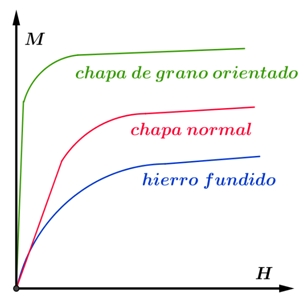
\includegraphics[width=0.60\textwidth]{./Figures/FerromagnetismoGranoOrientado.jpg}
	\caption{Magnetización en acero al Silicio, acero al carbono y fundición}
	\label{fig:FerromagnetismoGranoOrientado}
\end{figure}.


Para más detalles de la clasificación de los aceros se puede recurrir al sitio \url{https://www.ingemecanica.com/aceros/aceros01.html} donde se encontrarán las clasificaciones según las normas: ASTM, AISI, SAE, EN, CENIM y UNE. 


